\documentclass[12pt]{article}
%%% DOCUMENT FORMATTING %%%
\usepackage[margin=1in]{geometry}
\usepackage{enumitem}
\setlength{\parindent}{0pt}
\newcommand{\disp}{\displaystyle}

%%% HEADER %%%
\usepackage{fancyhdr}
\pagestyle{fancy}
\fancyhf{}
\lhead{MATH 1060}
\rhead{Vagnozzi}
\cfoot{\thepage}

%%% MATH NOTATION & SYMBOLS %%%
\usepackage{amssymb}
\usepackage{amsmath}
\newcommand{\R}{\mathbb{R}}
\newcommand{\N}{\mathbb{N}}
\newcommand{\Z}{\mathbb{Z}}
\newcommand{\lp}{\left(}
\newcommand{\rp}{\right)}
\newcommand{\ls}{\left[}
\newcommand{\rs}{\right]}
\newcommand{\lb}{\left\{}
\newcommand{\rb}{\right\}}
\newcommand{\arccot}{\text{arccot}}
\newcommand{\arccsc}{\text{arccsc}}
\newcommand{\arcsec}{\text{arcsec}} 

%%% TABLES %%%
\usepackage{colortbl}

%%% GRAPHS %%%
\usepackage{tikz}
\usepackage{pgfplots}
\pgfplotsset{compat=1.15}
\usepgfplotslibrary{fillbetween}
\usetikzlibrary{angles,quotes}

%%% ENVIRONMENTS %%%
\newcommand{\Example}{\paragraph{\Writinghand \hspace{0.1mm} Example.}}
\newcommand{\ExampleCont}{\paragraph{\Writinghand \hspace{0.1mm} Example (continued).}}
\newcommand{\boxenv}[2]{
	\fbox{
	\begin{minipage}{0.97\textwidth}
	\vspace{2mm}	
	\paragraph{#1} #2
	\vspace{2mm}
	\end{minipage}
	}}

%%% FUN THINGS %%%
\newcommand*\tc[1]{\tikz[baseline=(char.base)]{
            \node[shape=circle,draw,inner sep=2pt] (char) {#1};}}
\usepackage{marvosym}

%%% MISC %%%
\usepackage{hyperref}


\setcounter{page}{38}

\begin{document}
\section*{2.5: Limits at Infinity}

\boxenv{Learning Objectives.}{Upon successful completion of Section 2.5, you will be able to\dots
		
	\begin{itemize}[leftmargin=6mm]
		\item Evaluate limits at infinity.
		\item Answer conceptual questions involving end behavior and horizontal asymptotes.
		\item Find horizontal and vertical asymptotes of functions.
		\item Find slant asymptotes and sketch graphs of rational functions.
		\item Determine end behavior of transcendental functions and sketch their graphs.
		\item Solve applications involving limits used to find steady states.
		\item Sketch graphs of functions given information about end behavior.
	\end{itemize}
	\vspace{-4mm}
}

\vspace{5mm}

\subsection*{Introduction to Limits at Infinity}

In a \textbf{limit at infinity}, the independent ($x$) value is allowed to become boundless in either the positive or negative direction. If we attempt direct substitution in such limits, we often see the $\frac{\infty}{\infty}$ indeterminate form. Limits at infinity example the ``end behavior'' of a function.

\vspace{5mm}

\textbf{Example.} Consider again the function $f(x)=\disp\frac{1}{x}$.

\vspace{3mm}

\begin{center}
\begin{tabular}{|
>{\columncolor[HTML]{CBCEFB}}c |c|c|c|c|c|c|}
\hline
$x$   & 10 & 100 & 1,000 & 10,000 & 100,000 & 1,000,000 \\ \hline
$1/x$ & 0.1  & 0.01   & 0.001   & 0.0001  & 0.00001  & 0.000001  \\ \hline
\end{tabular}
\end{center}

As $x\to\infty$, $\disp\frac{1}{x}\to 0$. In other words, $\disp\lim_{x\to\infty}\frac{1}{x}=0$.

\vspace{3mm}

We could similarly show that $\disp\lim_{x\to -\infty}\frac{1}{x}=0$.

\begin{center}
            \begin{tikzpicture}[scale=1]
                \begin{axis}[
                	axis x line=middle,
                	xmax=4.2, xmin=-4.2,
                	axis y line=center,
                	ymax=4.2, ymin=-4.2,
                	xlabel=$x$,ylabel=$y$,
                	axis line style={<->}
                    ]
                    \addplot[name path=f,smooth,domain=-4:-0.25,color=blue,samples=100,thick,<->] {x^(-1)};
                    \addplot[name path=f,smooth,domain=0.25:4,color=blue,samples=100,thick,<->] {x^(-1)};
                     \draw (2.5,2) node[anchor=south] {\color{blue} $f(x)=\frac{1}{x}$};

                \end{axis}
            \end{tikzpicture}
        \end{center}

\subsection*{Horizontal Asymptotes}

\boxenv{Definition}{We say that $f$ is \textbf{asymptotic} to $g$ if and only if

$$\lim_{x\to\pm\infty}\vert f(x)-g(x)\vert=0$$

where $f$ and $g$ are any two functions defined as $x\to\infty$.}

\vspace{3mm}

\boxenv{Definition.}{The line $y=L$ is called a \textbf{horizontal asymptote} (H.A.) if and only if $\disp\lim_{x\to\pm\infty}f(x)=L$ where $L\in\R$.

\vspace{-1mm}}

\vspace{5mm}

\textbf{Example.} The inverse tangent function has horizontal asymptotes at $y=\frac{\pi}{2}$ and $y=-\frac{\pi}{2}$.

\begin{center}
            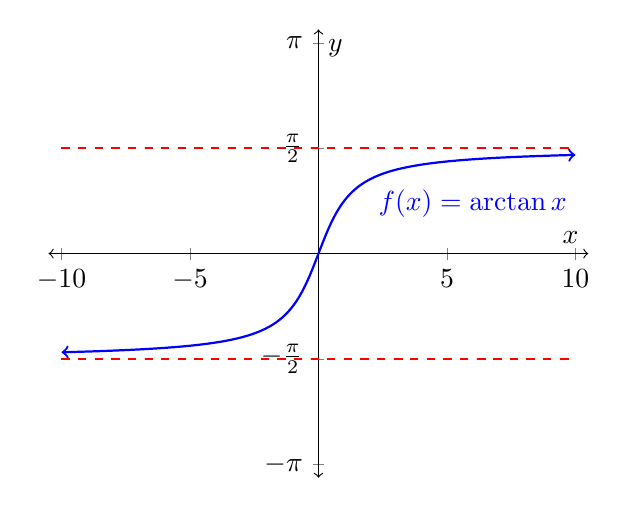
\begin{tikzpicture}[scale=1]
                \begin{axis}[
                	axis x line=middle,
                	xmax=10.5, xmin=-10.5,
                	axis y line=center,
                	ymax=pi+.2, ymin=-pi-.2,
                	xlabel=$x$,ylabel=$y$,
					ytick={-pi,-pi/2,0,pi/2,pi},
                	yticklabels={$-\pi$,$-\frac{\pi}{2}$,0,$\frac{\pi}{2}$,$\pi$},
                	axis line style={<->}
                    ]
                    \addplot[name path=f,smooth,domain=-10:10,color=blue,samples=100,thick,<->] {rad(atan(x))};
                    \addplot[name path=f,smooth,domain=-10:10,color=red,dashed,samples=100,thick] {pi/2};
                    \addplot[name path=f,smooth,domain=-10:10,color=red,dashed,samples=100,thick] {-pi/2)};
                    \draw (6,.4) node[anchor=south] {\color{blue} $f(x)=\arctan x$};

                \end{axis}
            \end{tikzpicture}
        \end{center}
        
\Example If $k\in\R$, $k\neq 0$, evaluate the limit $\disp\lim_{x\to\infty}\frac{1}{k}\arctan x$.

\newpage

\Example Evaluate the following limit.

\vspace{5mm}

\hspace{10mm} $\disp\lim_{x\to -\infty}\frac{3e^{-x}-1}{2e^{-x}}$

\vspace{50mm}

\paragraph{Polynomials.}\phantom{line break}

\vspace{3mm}

\boxenv{Definition.}{A \textbf{polynomial} is a function of the form

$$f(x)=a_n x^n+a_{n-1}x^{n-1}+a_{n-2}x^{n-2}+\cdots+a_0$$

where each $a_i\in \R$ and each power is a nonnegative integer, i.e.\ $\lb0,1,2,3,\dots\rb$. The domain and range of every polynomial is $\R$.}

\vspace{5mm}

\textbf{Examples.}
\begin{itemize}
	\item $f(x)=3x^6+2x^4+x^2-5$ is a polynomial.
	\item $g(x)=3x^{-1}+2x^2-3x$ is not a polynomial (negative exponent).
	\item $h(x)=x^2+x^\frac{1}{2}$ is not a polynomial (fractional exponent).
\end{itemize}

\vspace{3mm}

Polynomials have the following properties for limits at infinity.
\begin{itemize}
	\item $\disp\lim_{x\to\pm\infty}x^n=\infty$ when $n$ is even.
	\item $\disp\lim_{x\to\infty}x^n=\infty$ and $\disp\lim_{x\to -\infty}x^{n}=-\infty$ when $n$ is odd.
	\item $\disp\lim_{x\to\pm\infty}\frac{1}{x^n}=\lim_{x\to\pm\infty}x^{-n}=0$.
	\item If $p$ is any polynomial, then $\disp\lim_{x\to\pm\infty}p(x)=\pm\infty$.
\end{itemize}

\newpage

\Example Evaluate the following limit.

\vspace{5mm}

\hspace{10mm} $\disp\lim_{x\to -\infty}\lp 3x^{-7}+7x^3\rp$

\vspace{50mm}

\textbf{Rational Functions.}

\vspace{3mm}

\boxenv{Definition.}{A \textbf{rational function} is a function of the form 

$$Q=\frac{f(x)}{g(x)},$$

where $f$ and $g$ are polynomials. The domain of rational functions is $\R$ excluding the $x$-values that make $g(x)=0$.}

\vspace{3mm}

\boxenv{Remark.}{If a rational function has a horizontal asymptote, it only has one.}

\vspace{5mm}

To find the horizontal asymptote(s) of a rational function, we evaluate the limits at infinity by dividing each term of the function by the highest degree term of the denominator.

\Example Find the horizontal asymptote(s) of $f(x)=\disp\frac{2x^3+7}{3x^3-x^2+x+7}$.

\newpage 

\Example Evaluate the following limit.

\vspace{5mm}

\hspace{10mm} $\disp\lim_{x\to\infty}\frac{2x^4+5}{3x^3-2x^2+7}$

\vspace{50mm}

\Example Evaluate the following limit.

\vspace{5mm}

\hspace{10mm} $\disp\lim_{x\to -\infty}\frac{2x^4-3x}{3x^5+2x^2}$

\vspace{50mm}

\textbf{Limits at Infinity with Absolute Values.} Consider the function $\sqrt{x^2}$ and note the following.
\begin{center}
If $x=-1$, then $\sqrt{(-1)^2}=\sqrt{1}=1$.

\vspace{3mm}

If $x=1$, then $\sqrt{1^2}=\sqrt{1}=1$.
\end{center}

Here we see that $\sqrt{x^2}$ behaves like $\vert x \vert$, the absolute value function, which can be defined as a piecewise function.

$$ \sqrt{x^2} = \vert x \vert = \begin{cases} +x & x \geqslant 0 \\ -x & x < 0 \end{cases} $$

\newpage

\begin{center}
\fbox{\color{blue} $f(x)=\sqrt{x^2}=\vert x \vert$}

\vspace{3mm}

            \begin{tikzpicture}[scale=1]
                \begin{axis}[
                	axis x line=middle,
                	xmax=5, xmin=-5,
                	axis y line=center,
                	ymax=5, ymin=-1,
                	xlabel=$x$,ylabel=$y$,
                	axis line style=<->
                    ]
                    \addplot[name path=f,smooth,domain=0:4.5,color=blue,samples=200,thick,->] {x};
                    \addplot[name path=f,smooth,domain=-4.5:0,color=blue,samples=200,thick,<-] {-1*x};
                   
                \end{axis}
            \end{tikzpicture}
        \end{center}
        
\Example Evaluate the following limit.

\vspace{5mm}

\hspace{10mm} $\disp\lim_{x\to-\infty}\frac{2x+5}{\sqrt{2x^2+5x}}$

\vspace{48mm}

\subsection*{Oblique Asymptotes}

\vspace{3mm}

\boxenv{Definition.}{An \textbf{oblique asymptote} of a rational function $Q$ is a polynomial $\mathcal{O}$ of degree greater than or equal to one such that

$$\lim_{x\to\pm\infty}\vert Q(x)-\mathcal{O}(x)\vert=0,$$

i.e.\ the distance between $Q$ and $\mathcal{O}$ vanishes as $x\to\pm\infty$.}

\vspace{3mm}

\boxenv{Theorem.}{An oblique asymptote exists only when the degree of the numerator of $Q$ is greater than the degree of the denominator of $Q$.}

\vspace{3mm}

\boxenv{Remark.}{For a rational function, an oblique asymptote and a horizontal asymptote may not coexist.}

\newpage

\paragraph{How to Find Oblique Asymptotes.} We can perform \textit{polynomial long division} on a rational function $Q$ in order to obtain $Q(x)=\mathcal{O}(x)+R(x)$, where $\mathcal{O}$ is the quotient and $R$ is the remainder, which may not necessarily be zero. We can then show that 

$$\lim_{x\to\pm\infty}\vert R(x)\vert=0\,\Longleftrightarrow \,\lim_{x\to\pm\infty}\vert Q(x)-\mathcal{O}(x)\vert =0,$$

\vspace{2mm}

which implies that $\mathcal{O}$, the \textbf{quotient} of the polynomial long division, is the oblique asymptote.

\vspace{5mm}

\boxenv{Remark.}{If the degree $n$ of the numerator and degree $k$ of the denominator differ by one, i.e.\ $n-k=1$, then the oblique asymptote is a line and may be referred to as a \textbf{slant asymptote}.}

\vspace{5mm}

\Example Find all asymptotes of $f(x)=\disp\frac{x^4+x^3+x}{x+1}$.

\vspace{70mm}

\begin{center}
\fbox{\color{blue} $f(x)=\disp\frac{x^4+x^3+x}{x+1}$}

\vspace{5mm}

            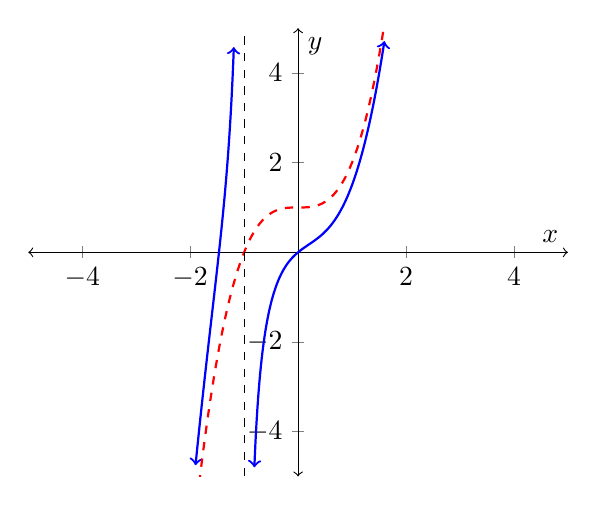
\begin{tikzpicture}[scale=1]
                \begin{axis}[
                	axis x line=middle,
                	xmax=5, xmin=-5,
                	axis y line=center,
                	ymax=5, ymin=-5,
                	xlabel=$x$,ylabel=$y$,
                	axis line style=<->
                    ]
                    \addplot[name path=f,smooth,domain=-1.9:-1.19,color=blue,samples=100,thick,<->] {(x^4+x^3+x)/(x+1)};
                    \addplot[name path=f,smooth,domain=-0.81:1.6,color=blue,samples=100,thick,<->] {(x^4+x^3+x)/(x+1)};
                    \addplot[name path=f,smooth,domain=-5:5,color=red,dashed,samples=100,thick,<->] {x^3+1};
    \draw [dashed] (-1,-5) -- (-1,5);
                \end{axis}
            \end{tikzpicture}
        \end{center}
        
\newpage 

\subsection*{End Behavior of Other Notable Functions}

\vspace{5mm}

            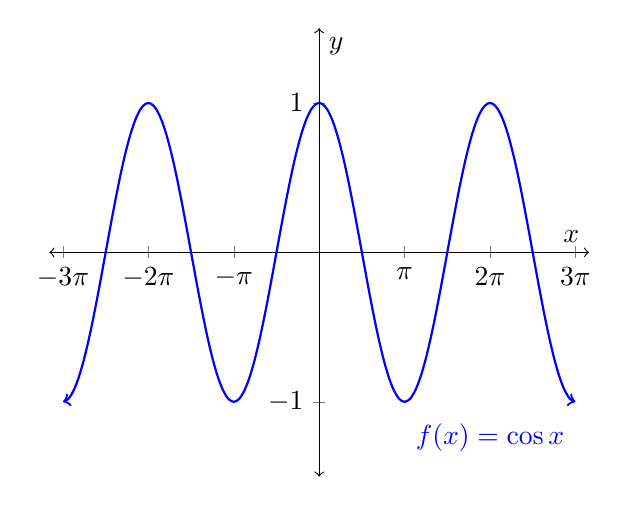
\begin{tikzpicture}[scale=1]
                \begin{axis}[
                	axis x line=middle,
                	xmax=3*pi+.5, xmin=-3*pi-.5,
                	axis y line=center,
                	ymax=1.5, ymin=-1.5,
                	xlabel=$x$,ylabel=$y$,
                	xtick={-3*pi,-2*pi,-pi,0,pi,2*pi,3*pi},
                	xticklabels={$-3\pi$,$-2\pi$,$-\pi$,$0$,$\pi$,$2\pi$,$3\pi$},
                	axis line style={<->}
                    ]
                    \addplot[name path=f,smooth,domain=-3*pi:3*pi,color=blue,samples=100,thick,<->] {cos(deg(x))};
                    \draw (2*pi,-1.4) node[anchor=south] {\color{blue} $f(x)=\cos x$};

                \end{axis}
            \end{tikzpicture}
        
        \vspace{5mm}
        
            \begin{tikzpicture}[scale=1]
                \begin{axis}[
                	axis x line=middle,
                	xmax=5.2, xmin=-1.2,
                	axis y line=center,
                	ymax=4.2, ymin=-4.2,
                	xlabel=$x$,ylabel=$y$,
                	axis line style={<->}
                    ]
                    \addplot[name path=f,smooth,domain=0.01:4.5,color=blue,samples=300,thick,<->] {ln(x)};
                    \draw (1.5,1.5) node[anchor=south] {\color{blue} $f(x)=\ln x$};

                \end{axis}
            \end{tikzpicture}

\vspace{5mm}

            \begin{tikzpicture}[scale=1]
                \begin{axis}[
                	axis x line=middle,
                	xmax=5, xmin=-5,
                	axis y line=center,
                	ymax=4.2, ymin=-1.2,
                	xlabel=$x$,ylabel=$y$,
                	axis line style={<->}
                    ]
                    \addplot[name path=f,smooth,domain=-5:1.36,color=blue,samples=200,thick,<->] {e^x};                    
                    \draw (3,1) node[anchor=south] {\color{blue} $f(x)=e^x$};

                \end{axis}
            \end{tikzpicture}
        
        \vspace{5mm}
        
        \newpage

\subsection*{Summary}

\paragraph{Rational Functions at Infinity.} For a rational function $f(x)$, let $n$ be the degree of the numerator and $k$ be the degree of the denominator.
\begin{itemize}
	\item If $n<k$ (i.e.\ if the function is ``bottom-heavy''), then $f(x)$ will approach zero.
	\item If $n>k$ (i.e.\ if the function is ``top-heavy''), then $f(x)$ will approach $\pm\infty$. 
	\item If $n=k$, then $f(x)$ will approach the ratio of the leading coefficients of the numerator and denominator.
\end{itemize}

\paragraph{Asymptotes of a Function.}
\begin{itemize}
	\item A function has a \textbf{vertical axis} (V.A.) at $x=c$ if the denominator only is zero and any limit of $f(x)$ as $x\to c$ is $\pm \infty$.
	\item A function has a \textbf{horizontal asymptote} (H.A.) at $y=L$ if $\disp\lim_{x\to\pm\infty}f(x)=L$.
	\item A function has an \textbf{oblique asymptote} (O.A.) at the quotient $\mathcal{O}(x)$ found by performing polynomial long division.
\end{itemize}
\end{document}